\documentclass[letter]{sig-alternate}
\usepackage{epsfig}
\usepackage{graphicx}
\usepackage{amsmath}
\usepackage{amssymb}
\usepackage{algorithm}
\usepackage{algorithmic}
\usepackage{subfigure}
\usepackage{url}
\usepackage{multirow}
\usepackage[usenames,dvipsnames,table]{xcolor}

\begin{document}

\conferenceinfo{MM'12,} {October 29--November 2, 2012, Nara, Japan.} 
\CopyrightYear{2012} 
\crdata{978-1-4503-1089-5/12/10} 
\clubpenalty=10000 
\widowpenalty = 10000

%
% --- Author Metadata here ---
%\conferenceinfo{ACM MM'12}{2012, Nara, Japan}

\title{Eheritage: Shadow Puppetry Creation and Manipulation}
%\subtitle{[Extended Abstract]
%\titlenote{A full version of this paper is available as
%\textit{Author's Guide to Preparing ACM SIG Proceedings Using
%\LaTeX$2_\epsilon$\ and BibTeX} at
%\texttt{www.acm.org/eaddress.htm}}}






\numberofauthors{1} 
\author{\alignauthor Zhenzhen Hu, Min Lin, Si Liu$^{1,2}$, Richang Hong, Wang Meng,   Shuicheng Yan$^{1}$ \\
\affaddr{\small $^{1}$ ECE Department, National University of Singapore}   \\
\affaddr{\small $^{2}$ School of Computer and Information, Hefei University of Technology}   \\
\affaddr{\tt\small \{a0104018,dcslius,eleyans\}@nus.edu.sg}
} 


\maketitle
\begin{abstract}
In this paper, we propose a creative and manipulable Chinese shadow play system to automatically create user-specified shadow puppetry figure and manipulate figure to tell story by user script. 

\end{abstract}




% A category with the (minimum) three required fields
%\category{H.3.3}{Information Search and Retrieval}{Retrieval models}
%A category including the fourth, optional field follows...

%\category{I.2.6 }{Learning}{Knowledge acquisition}

\terms{Algorithms, Experimentation, Performance}

\keywords{Chinese shadow puppetry, face rendering, dynamic programming, SVM}





\section{Introduction}

Chinese shadow puppetry is a traditional graphical art which describes a story with a sequence of puppetry images. It is a kind of drama that silhouettes made of hard leather and projected onto a white screen. As an ancient form of storytelling, puppets are manipulated in sticks and flat behind an illuminated background to create moving pictures \cite{chen2012visions}. By moving both the puppets and the light source, various effects can be achieved. 

A traditional Chinese shadow puppetry is composed by a head part and a body part.The design of the figures follows traditional moral evaluation and aesthetics. The audience can tell a figure's character by seeing his mask. A red mask represents uprightness, a black mask, fidelity, and a white one, treachery. The positive figure has long narrow eyes, a small mouth and a straight bridge of nose, while the negative one has small eyes, a protruding forehead and sagging mouth. The procedure of puppet making include nearly seven steps which are all complex and ingenious. Nowadays, few existing shadow puppets have been collectible curiosities. To create a personal shadow puppet is 

The performance pattern of Chinese shadow puppetry is also varied. A talented puppeteer can make the figures perform all kinds of actions, such as walk, dance, fight, nod and laugh. However, it is not that easy for a normal user to control the movements of the puppets. A more friendly interface for them is to manipulate directly using input text script so that the puppets can play the motions with user director.





\begin{figure}[t]
\begin{center}
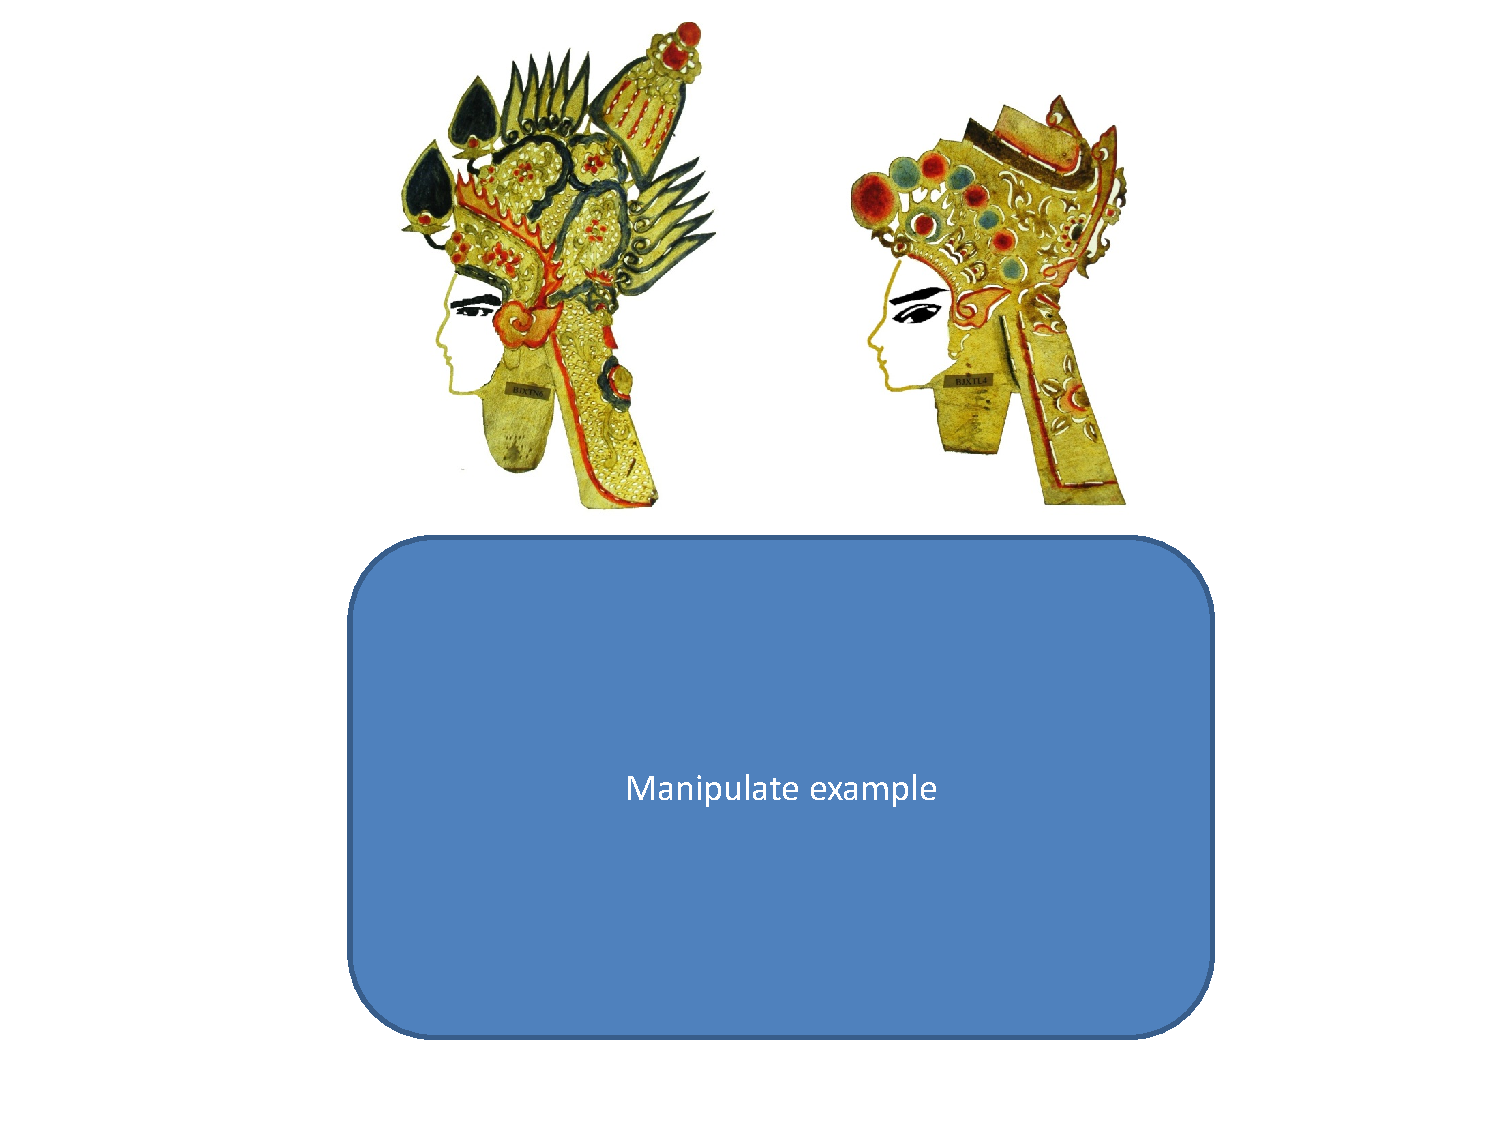
\includegraphics[scale=0.4]{figure/SyetemIntro.pdf}
\caption{\small{system introduction.}}
\label{fig:firstfig}
\end{center}
\end{figure}

Digital puppetry technique has received lots of interests in the past years. To solve the complex operation skills, existing researches on shadow puppets are focus on the user body interaction capabilities for controlling the puppets  \cite{leite2012shape},\cite{lin2012action},\cite{zhang2012chinese}.
Control the puppetry motion by human body is activity. However, the real puppet is controlled by simple three sticks which fixed on puppetry neck and two hands separately, and its motion pattern affected by gravity has special styles. (Here is a figure) Puppetry techniques mentioned above can't guarantee the puppetry motion style. So these kinds of play cannot convey this traditional art charm completely.

Our artistic motivation is to exploit a system in which the shadow puppetry becomes fully creative and more manipulable naturally.In this paper, we propose a creative and manipulable shadow play system to automatically create user-specified shadow puppetry figure and manipulate figure to tell story by user script. Our approach mainly contains two aspects: creation and manipulation. For creation, we extract the central profile curve from side view face image and warp front view eye into puppet eye style simultaneously. Then we transfer the texture of face area into puppet texture. For manipulation ,XXX.

Our objective is to create a digital puppetry figure used with non expert-artists to create expressive virtual shadow plays using input script.

The remainder of paper is structured as follows.


\section{Related Work} \label{sec:related}


\begin{figure}[t]
\begin{center}
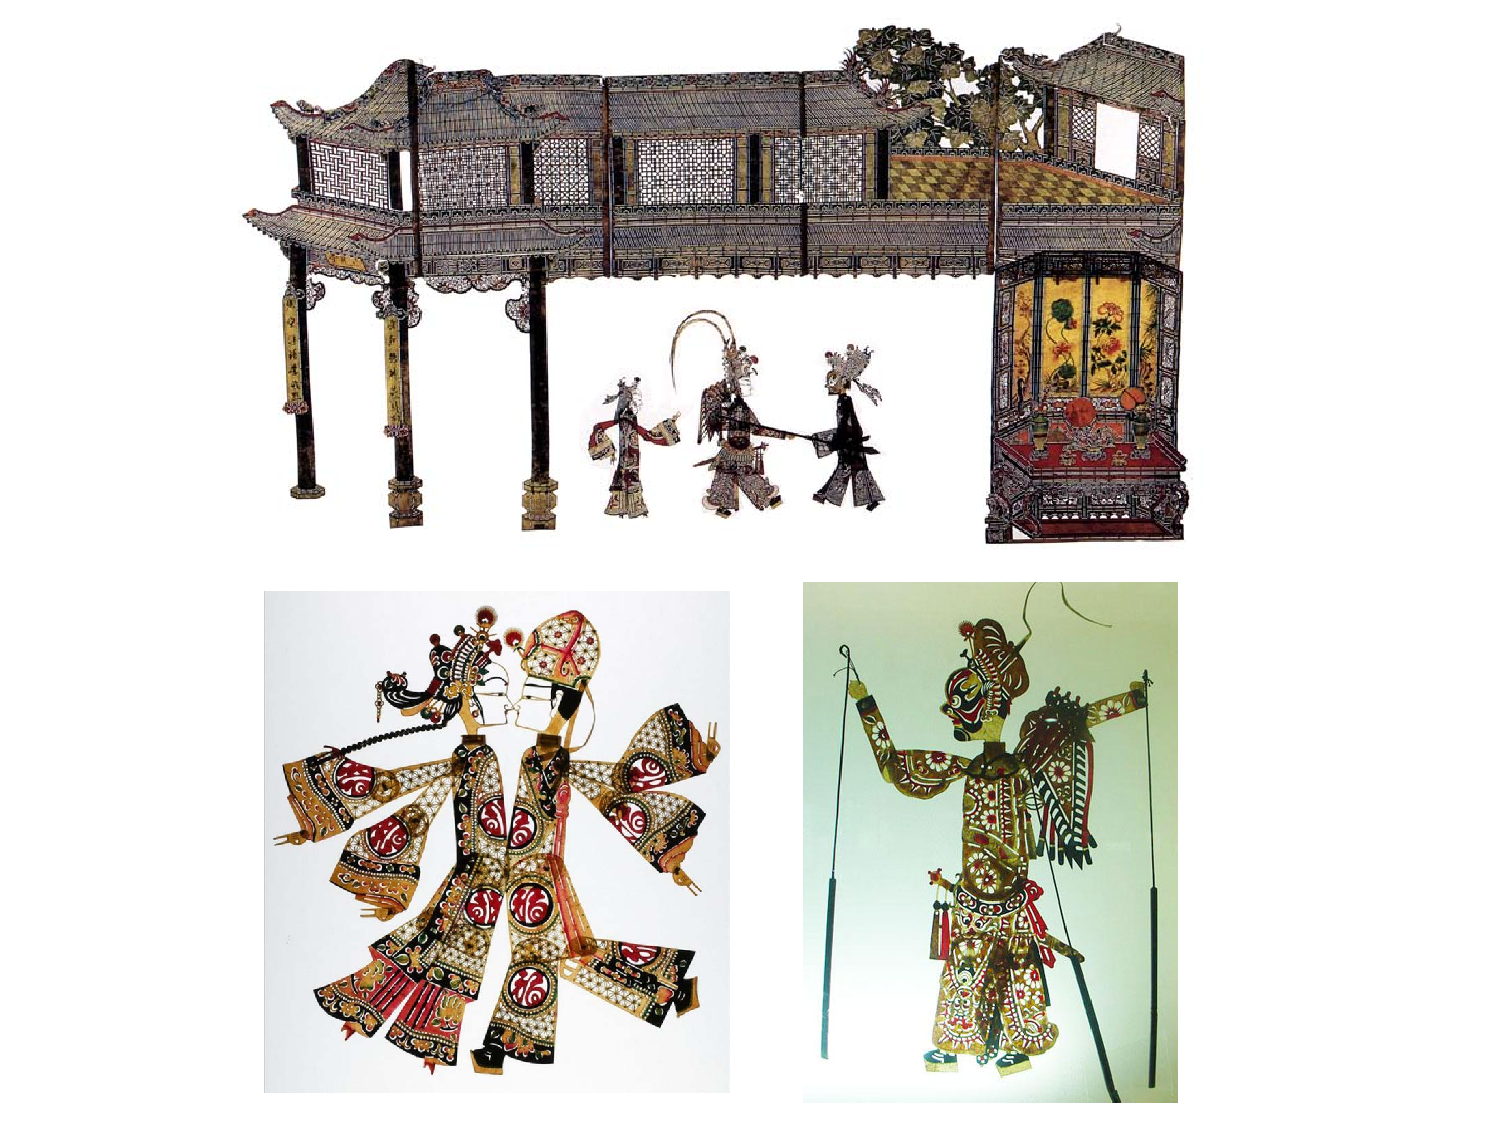
\includegraphics[scale=0.4]{figure/puppetru_introduction.pdf}
\caption{\small{puppetry introduction.}}
\label{fig:firstfig}
\end{center}
\end{figure}

\subsection{Face Rendering}

Digital image processing provides a solid foundation for building artistic rendering algorithms. All image-based artistic rendering (IB-AR) approaches utilize image processing operations in some form to extract information or synthesize results. For instance, classical stroke-based rendering utilizes the image gradient for stroke placement.

\subsection{Digital puppetry }

Digital puppetry experiments started in early 1960s, using analog circuits to animate figures in real-time, conducted by Lee Harrison III \cite{sturman1998state}. But it was only in 1988 that the live animated computer graphics (CG) characters arrived. Recently, a lot of works have been carried out on digital puppetry. 



However, all of these mentioned works are based on 3D characters. Shadow puppets are also used to produce animated films. The Adventures of Prince Achmed is an example of a feature film from 1962 built with thousands of cutout paper puppets, but producing an animated film with shadow puppets, frame by frame, is laborious and time-consuming.

The solution of animation performed by two dimensional puppets appears only recently.
In \cite{hsu2005planning}, Hsu et al. introduced a motion planning technique which automatically generates the animation of 2D puppets. Tan et al. \cite{tan2010real} presented a method for interactive animation of 2D shadow play puppets by real-time visual simulating the shadow using texture mapping, blending techniques, and lighting and blurring effects. ShadowStory \cite{lu2011shadowstory} is a project created by Fei et al. for digital storytelling inspired by traditional Chinese shadow puppetry. The system allows children to design with a tablet PC their own puppets and animate them. In \cite{pan2011sketch}, a 2D shape deformation of the triangulated cartoon is driven by its skeleton and the animation can be obtained by retargeting the skeleton joints to the shape.

We found interesting performance puppet manipulation methods in some digital puppet artwork, like Puppet Parade, an interactive puppetry installation that animates puppets by tracking the arms of the puppeteers, or We Be Monsters , a collaborative puppet art installation that tracks multiple skeletons to animate a puppet. Although they do not focus the shadow puppetry, they use the body motion to control the puppets.However, 













\section{Overview}

\begin{figure}[t]
\begin{center}
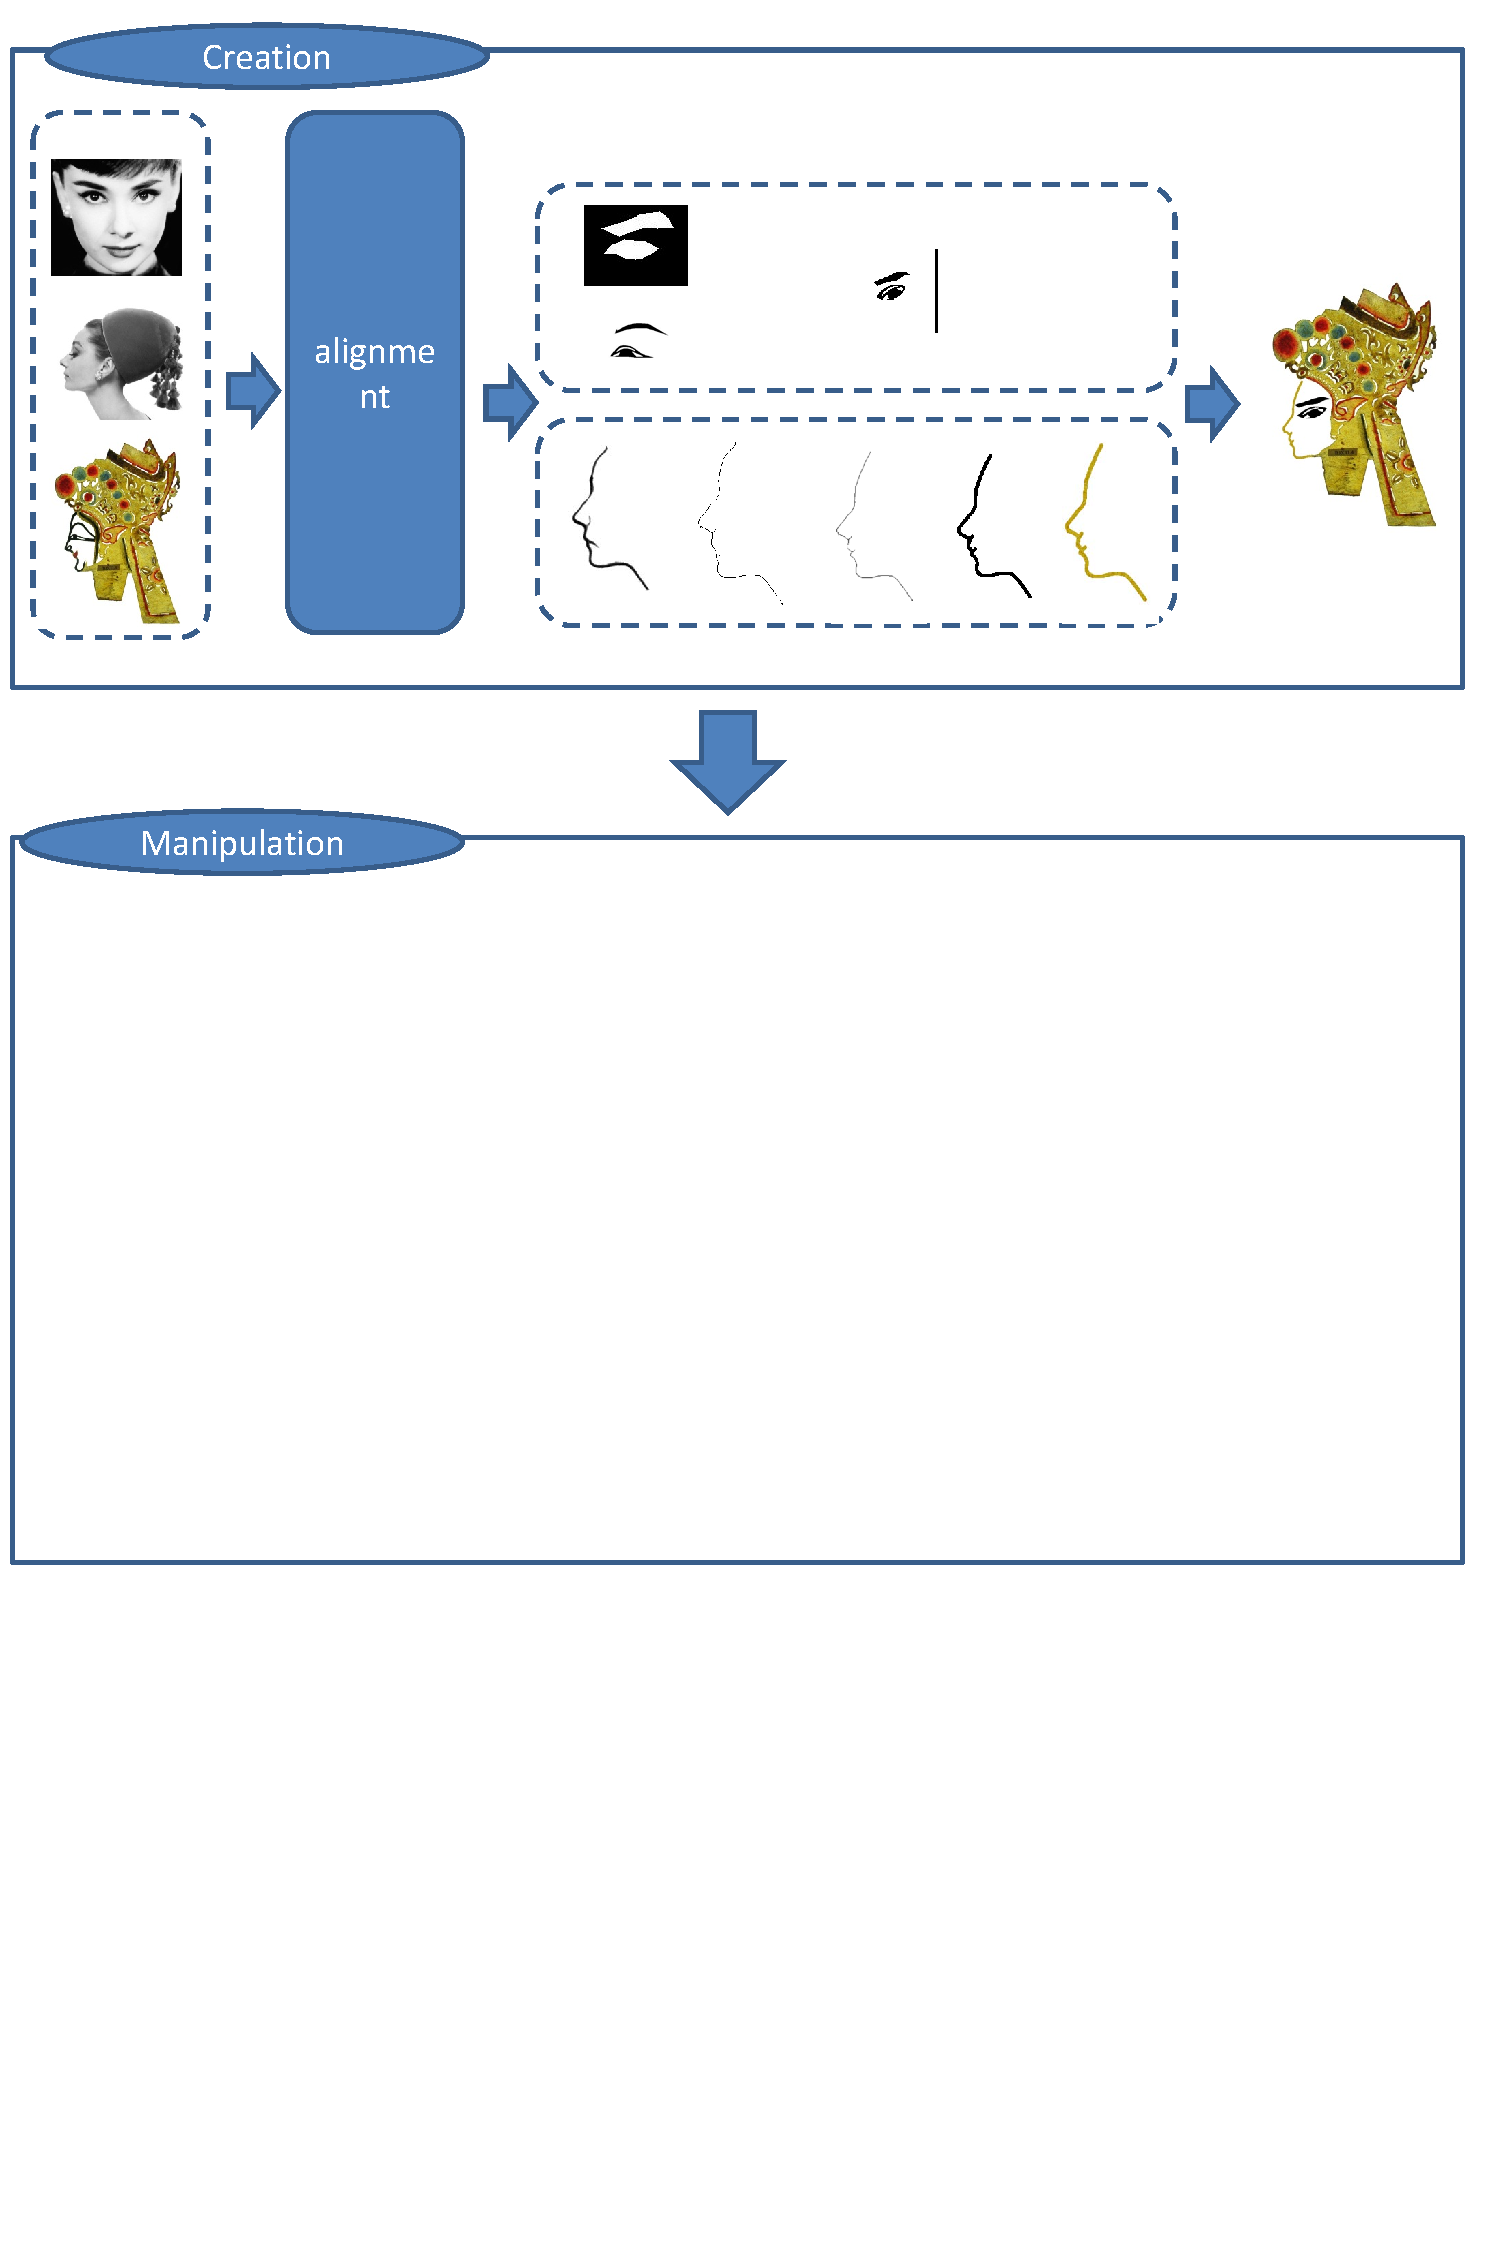
\includegraphics[scale=0.35]{figure/framework.pdf}
\caption{\small{Frame work}}
\label{fig:firstfig}
\end{center}
\end{figure}



\section{Puppetry API:  Creator}

The design of Chinese shadow puppetry figures follows traditional moral evaluation and aesthetics. There are mainly four kinds of puppetry face: Sheng (male roles), Dan (femal roles), Jing (roles with painted faces) and Chou (a comic character ). These roles are most from classical plays and appearances are formalization. Since the procedures of puppetry making is very complicated and expensive, user is hard to customize a specific puppetry figure. In this section, we will introduce the creation part of our system in details.

\subsection{Pre-Processing}

Given a front view face image and a side view face image of the same people, we use generally utilize front eye and eyebrow and side profile curve to creat a use-specified puppetry figure head.

Before creator, we aligned each face to the same direction ,rotated pictures according to Frankfort horizontal plane




%\begin{figure}[t]
%\begin{center}
%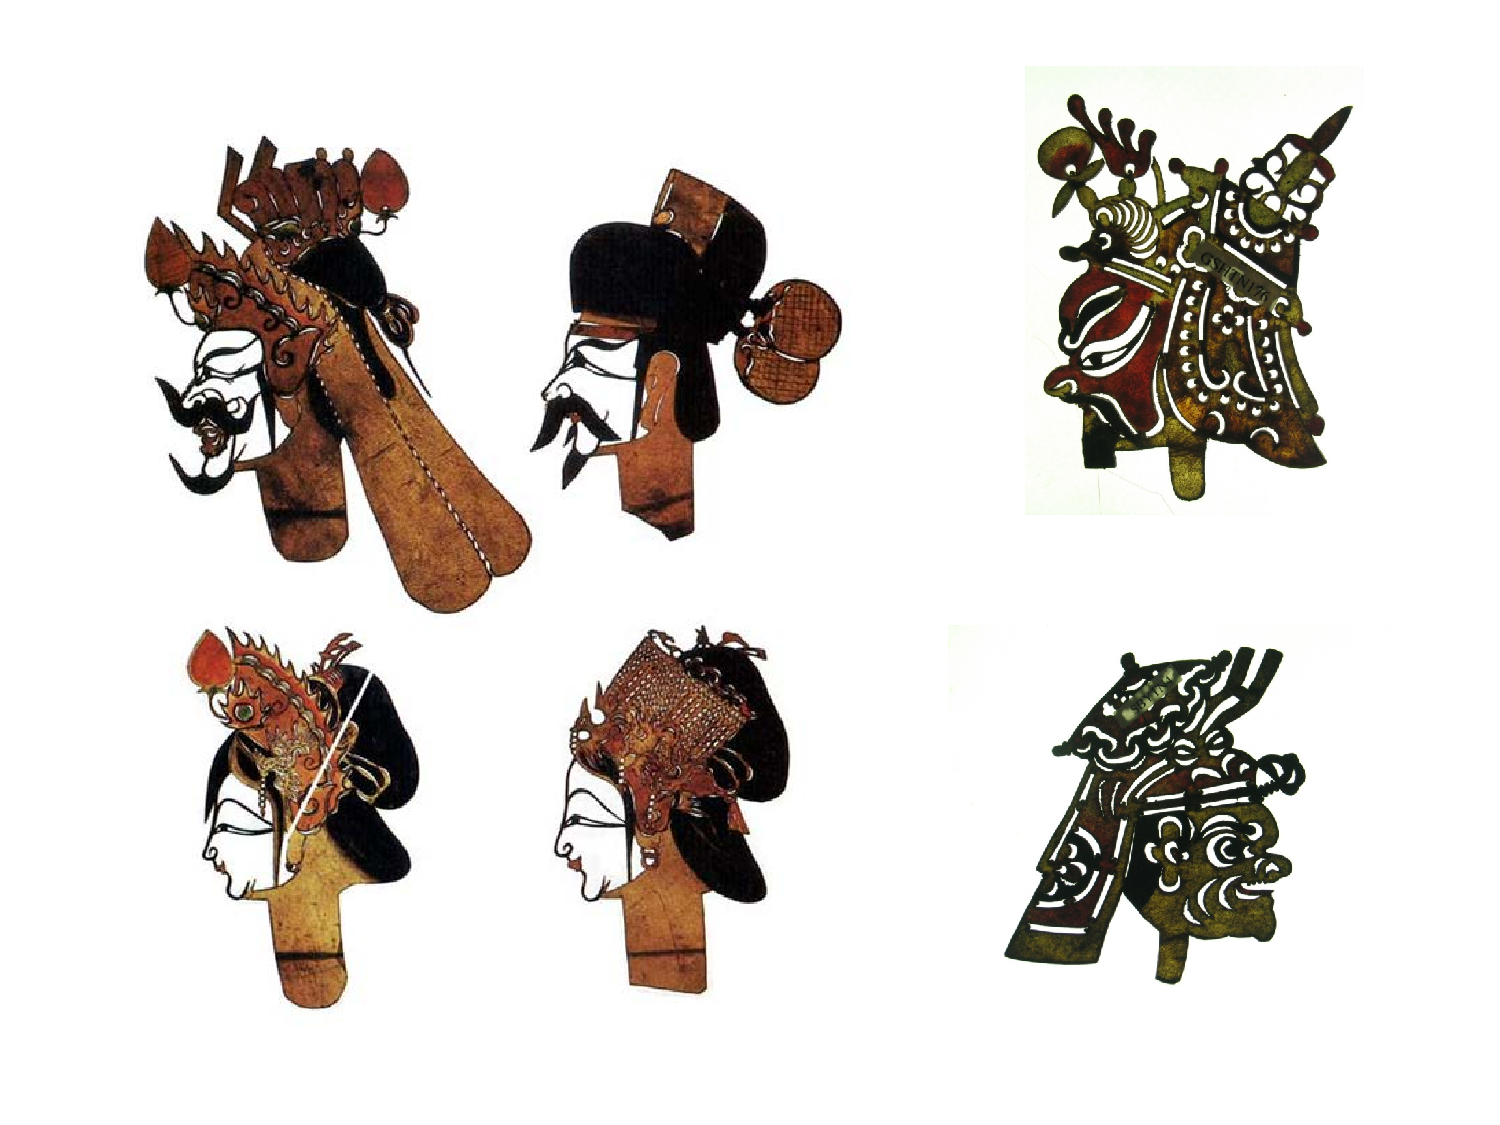
\includegraphics[scale=0.35]{figure/classify_intro.pdf}
%\caption{\small{puppetry classify}}
%\label{fig:firstfig}
%\end{center}
%\end{figure}

\subsection{Eye \& eyebrow warping}

In Chinese shadow puppetry, the face of figures are almost side-view. For the reason of  describing features of characters, eyes and eyebrow are abstracted and exaggerated in an artistic way. The topology of puppetry is similar to the front view eye. To guarantee the similarity of output figure face,  given an target front view face image and a puppetry face, we can warp the puppetry eye and eyebrow into target eye and eyebrow shape.

The key idea of most warping methods \cite{gomes1999warping,hormann2006mean} is that the user must provide an explicit correspondence between the source and target shapes. Other points are mapped according to their relative positions with respect to the correspondence (anchor) points. We would like the computer to derive this correspondence automatically. Barycentric coordinates for triangles provide a convenient way to linearly interpolate data that is given at the corners of a triangle. Given a planar triangle $\left[ v_{1},v_{2},v_{3}\right]$, any point $v$ inside it has three masses $w_{1}$, $w_{2}$ and $w_{3}$. If placed at the corresponding vertices of the  triangle, their barycentre will coincide with $v$:
\begin{equation}
 \dfrac {w_{1}v_{1}+w_{2}v_{2}+w_{3}v_{3}} {w_{1}+w_{2}+w_{3}}=v 
 \end{equation}
So $w_{1}$ ,$w_{2}$ and $w_{3}$ are defined as the barycentric coordinates of $v$.

Given an arbitrary planar polygon $\psi$ with vertices $\left\{v_{i}\right\}$, each point $x_{i}\in\psi$ has mean value coordinates corresponding to three vertices $v_{i-1}$, $v_{i}$ and $v_{i+1}$. For a topologically equivalent target polygon $\psi'$ with vertices $v_{i}'$, which $\psi$ and $\psi'$ have the same number of components and vertices for per component, we would like to construct a smooth warp function $f:\psi \rightarrow \psi'$ that maps each $v_{i}$ to $v_{i}'$. This warp function $f$ can then be used to deform the source image $I:x_{i}\in\psi$ into the target image $I':x_{i}'\in\psi'$ with new coordinates according to $v_{i-1}'$, $v_{i}'$ and $v_{i+1}'$.

According to our common sense, the shape of humane eye is convex. In our case, we first extract the contours of puppetry eye $C_i = \left\{ c_{1},\cdot \cdot\cdot , c_{n}\right\}$ and real eye $P_i = \left\{ p_{1},\cdot \cdot\cdot , p_{m}\right\}$,  by annotating landmarks around the eye boundary. In practice,we annotate 10 points, where $n=m=10$.

We define a warp from $C_i$ to $P_i$ by the approach introduced above, and apply it to the keywords. We apply the geometric warp of Hormann and Floater  \cite{hormann2006mean} inside each convex piece to obtain a warp of the entire phrase polygon. Each point in $C_i$ has the mean value coordinates according to vertices locations. When $C_i$ is warped to the location of $P_i$, a correspondence between the sample points on $C_i$ and $P_i$ can be generated. Given a correspondence between the sample points on $C_i$ and $P_i$, we can then map the points in polygon $C_i$ through the correspondence. 

%Some examples are shown in Figure~\ref{warpping}.




\begin{figure}[t]
\begin{center}
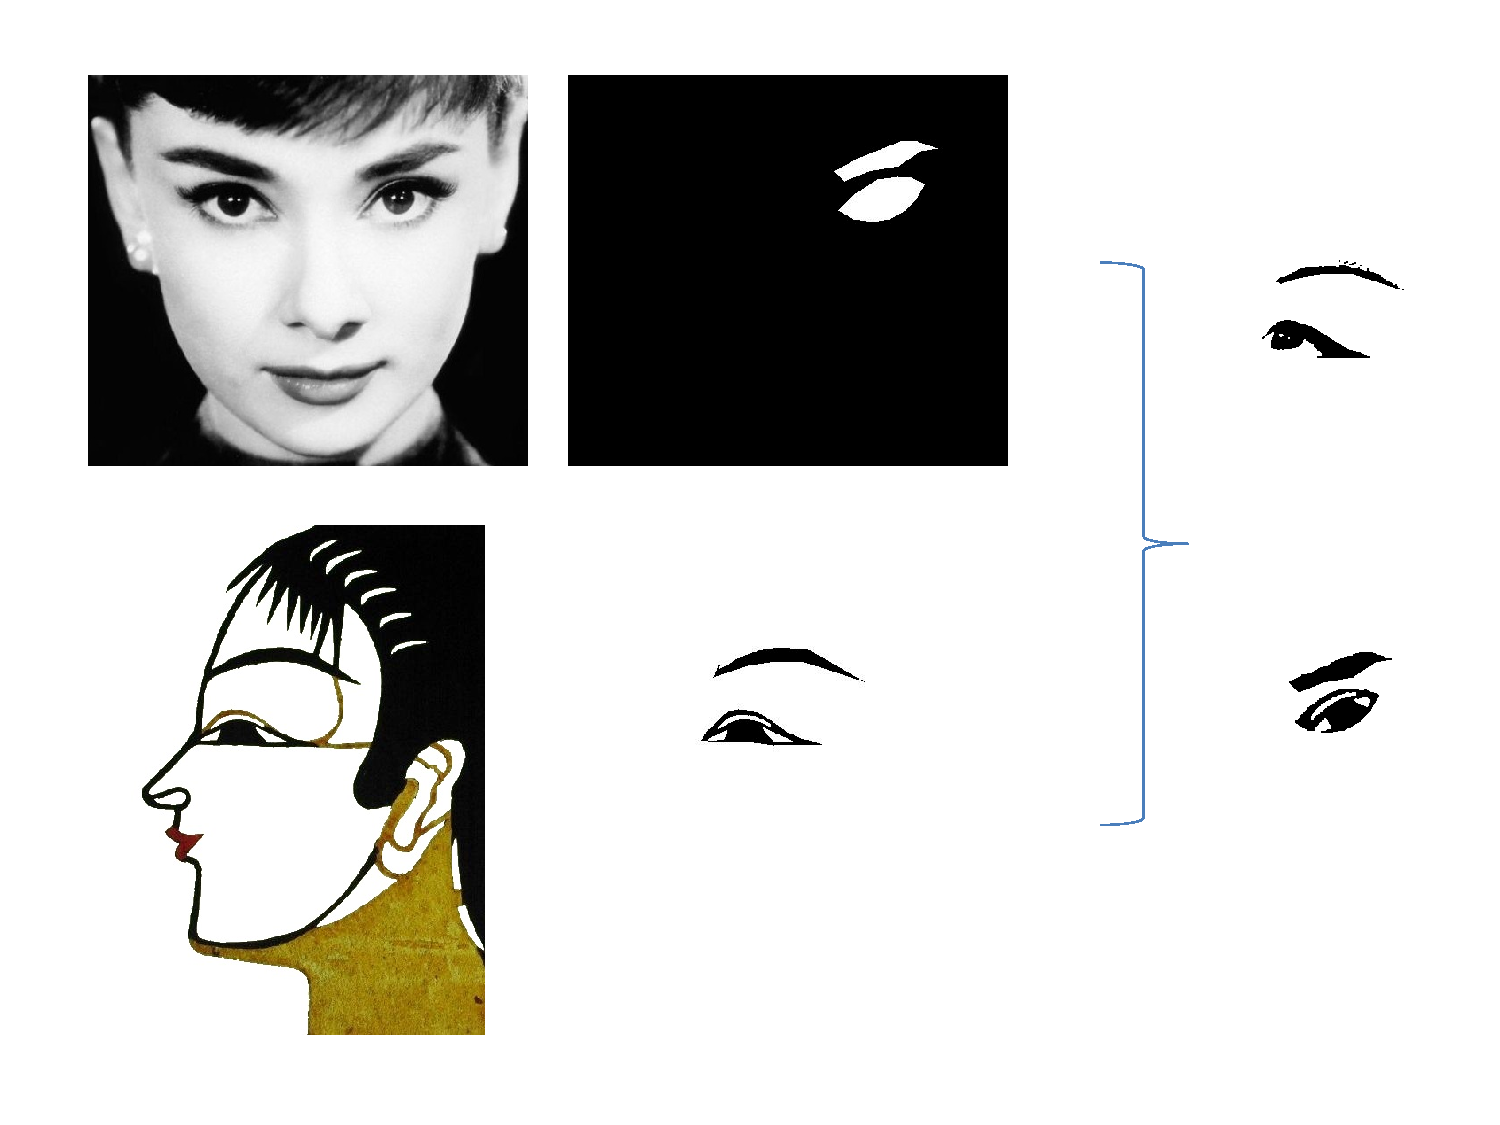
\includegraphics[scale=0.3]{figure/eyewarping.pdf}
\caption{\small{Eye \& eyebrow warping.}}
\label{fig:firstfig}
\end{center}
\end{figure}




\subsection{Profile Curve generation}
Central profile curve is an important geometric feature. To generate an appropriate puppetry profile, we will consider two aspects: 1) this profile shoule like the input face and 2) this profile should have puppetry style. we keep the most unique part of the profile curve and transfer it into puppetry style.


\begin{figure}[t]
\begin{center}
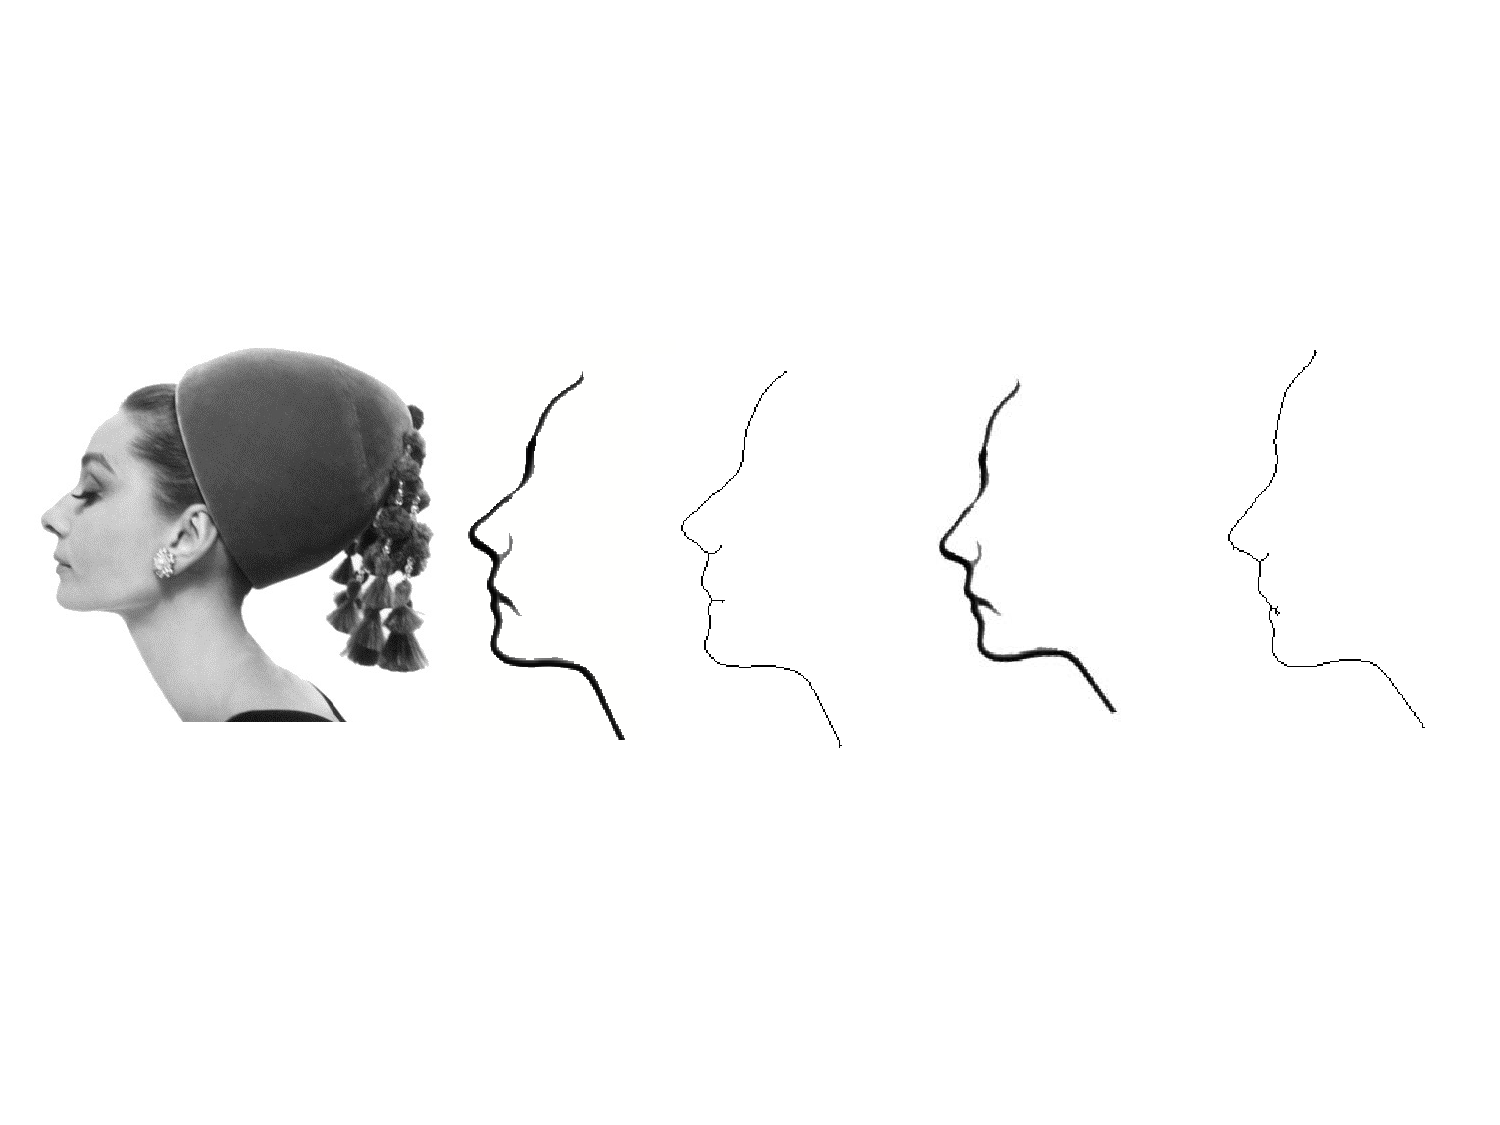
\includegraphics[scale=0.3]{figure/profile_abstract.pdf}
\caption{\small{Profile Curve generation.}}
\label{fig:firstfig}
\end{center}
\end{figure}
    



\subsubsection{Profile abstraction}

The central profile curve is highly discriminative. Some 3D facial research works use central profile curve as a significant feature to do face maching \cite{pan20033d} and face recognition \cite{nagamine19923d}.

Given a 90 degree side face, we first extract the edge of side view face according to \cite{winnemoller2011xdog} and detect the profile curve. Then we process this curve area by binary morphology tools and extract the skeleton line with only one pixel width. 

A profile curve can be separated into four parts: forehead, nose, mouth and jaw. For each part, we use histogram of oriented gradients (HOG) \cite{hog} to present the feature of this part with a vector. The uniqueness of each part is evaluated by a distance matrix of side-view face training dataset. We calculate the average distances between real face profile curves. The part which far from other training face is considered more unique. The two most unique parts are kept and the other parts are replaced by parts of shadow puppetry profile.


\subsubsection{Profile texture transfer}
After previous steps, we can generate a profile skeleton which both like real face and puppetry face. Then we dilate this line till puppetry profile width. To be more like puppetry, we transfer the leather texture to profile area. Alexei A. Efros \cite{efros2001image} presented a simple image quilting algorithm of generating novel visual appearance in which a new image is synthesized by stitching together small patches of existing images. Given a piece of leather sample in Figure, they synthesized the texture by following steps:

1) Go through the sample image in raster scan order in steps of one block.

2) For every location of binary profile image in Figure, search the input texture for a set of blocks that satisfy the overlap constraints within some error tolerance. 

3) Compute the error surface between the newly chosen block and the old blocks at the overlap region. Find the minimum cost path along this surface by dynamic programming and make that the boundary of the new block. Paste the block onto the texture. 

After image quilting, texture transfer is generated by requiring a desired correspondence map. The correspondence map is a spatial map of some corresponding quantity over both the texture source image and a controlling target image.

Some examples of texture transfer is shown in Figure 1.



\begin{figure}[t]
\begin{center}
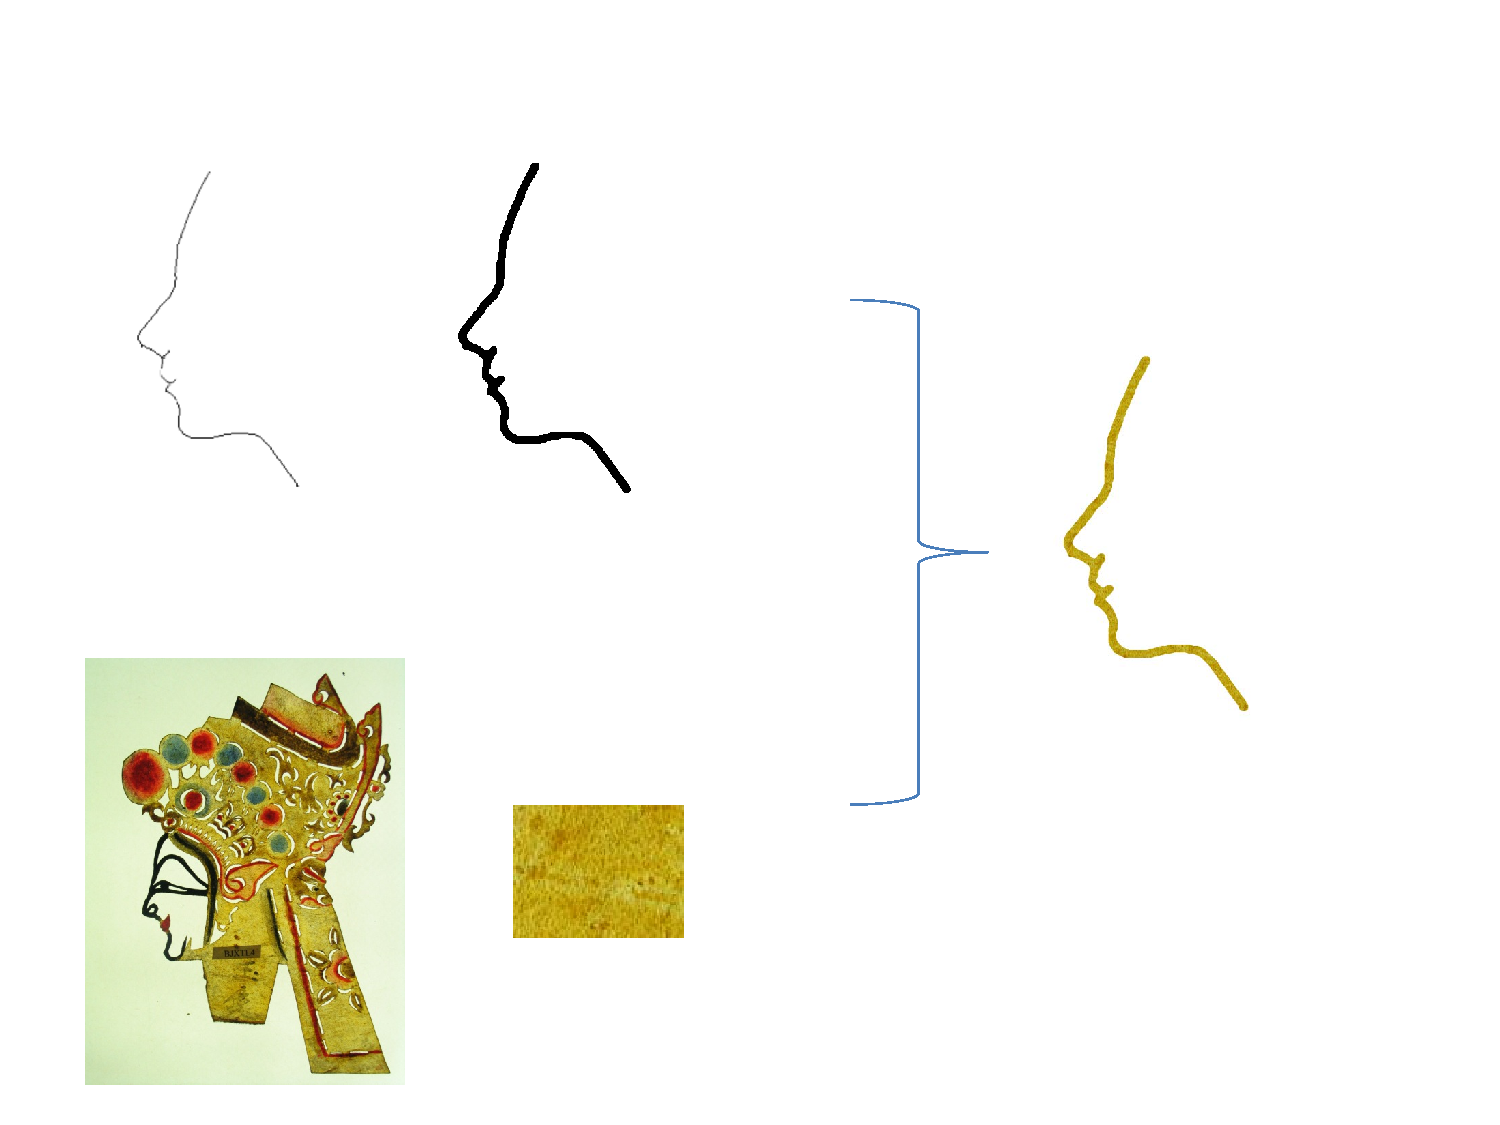
\includegraphics[scale=0.3]{figure/TextureTransfer.pdf}
\caption{\small{TextureTransfer}}
\label{fig:firstfig}
\end{center}
\end{figure}
    

\subsection{Post processing}
For artistically expressing roles of human, puppets are decorated with exquisite headdress. 

In shadow puppetry play, there is a lot of vivid props, including architecture, furniture, plants and animals, designed with distinct period features from past dynasties

\section{Puppetry API:  Manipulator}


Traditional Chinese shadow puppet is created by hinging together nine parts: head, body, left/right arm, left/right hand, lower body, front foot and rear foot, although there are variants replacing lower body with two upper legs, the nine-part design dominates. In a real puppet show, each puppet is controlled by three stick manipulators, the major manipulator is attached to neck, clipping together head and body. The other two manipulators each hinges to one hand. Based on this control model, shadow puppets has their own distinguished pattern of motion. In this section, we describe a system that is able to animate shadow puppet in their own style learned from real world puppet shows.

\begin{figure}[t]
\begin{center}
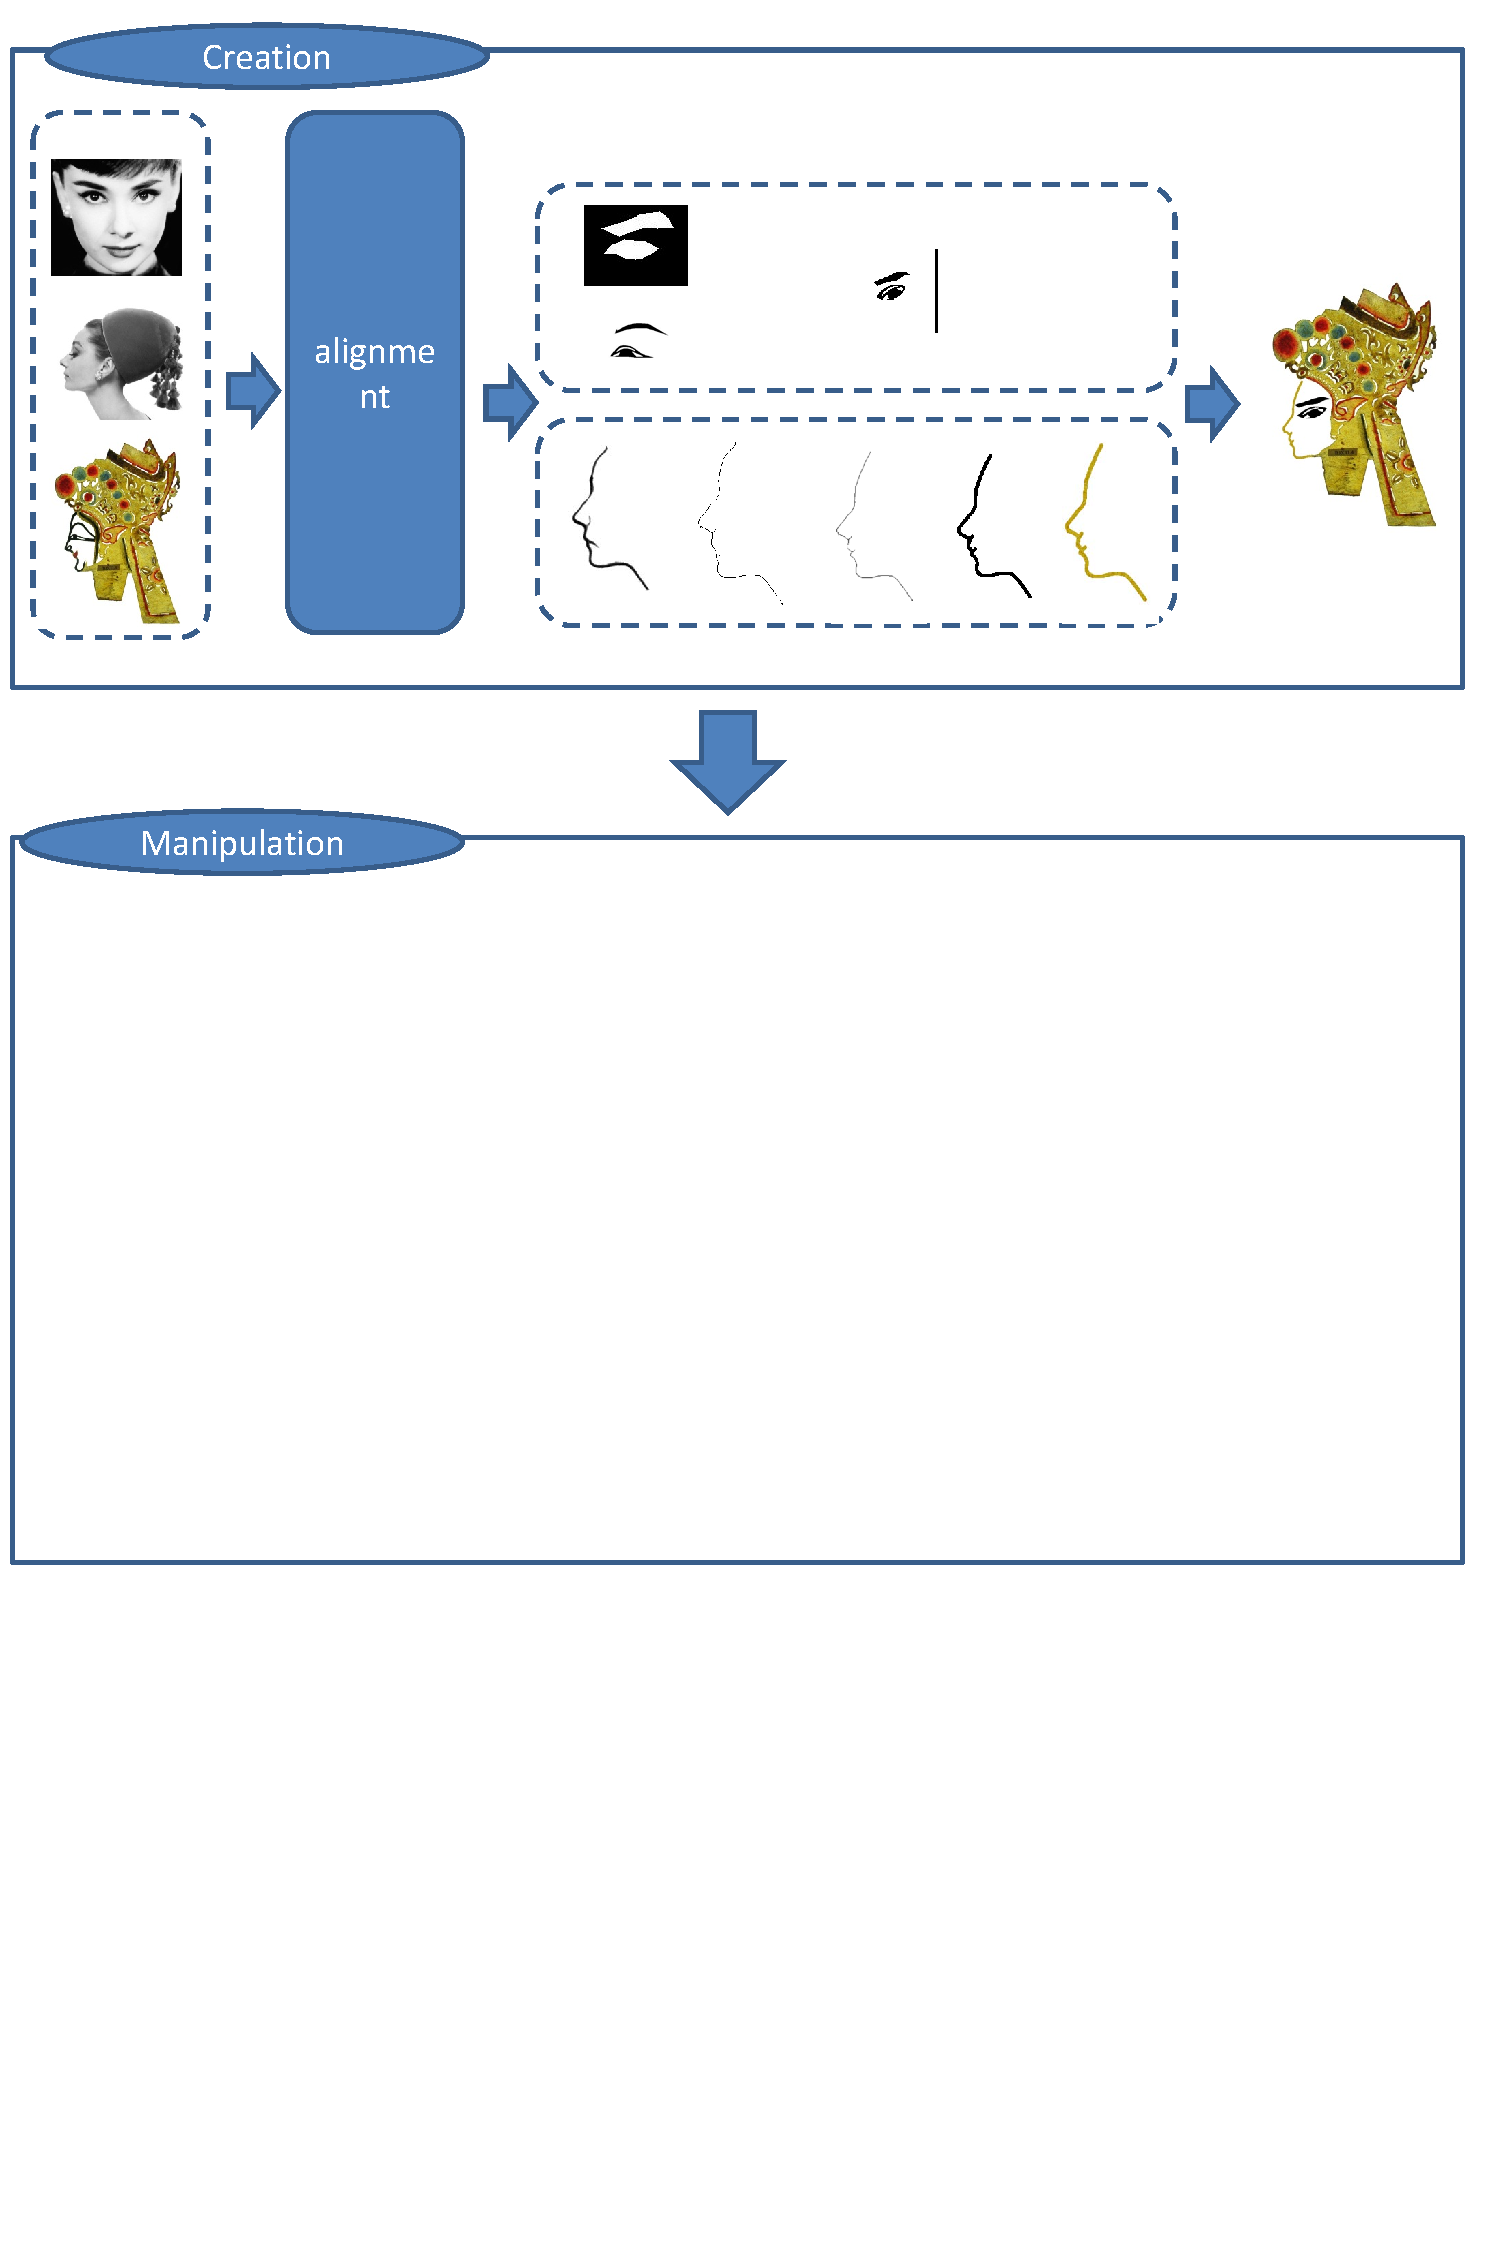
\includegraphics[scale=0.35]{figure/framework.pdf}
\caption{\small{degrees of freedom}}
\label{fig:degreeoffreedom}
\end{center}
\end{figure}

\subsection{Control model}
In our system we adopt the nine-part puppet design, each puppet character consists of nine parts, linked by seven joints and in total has 12 degrees of freedom (DOF), as depicted in figure~\ref{fig:degreeoffreedom}. The 7 joints are named according to their position, they are: left/right shoulder, left/right elbow, waist and front/rear knee. All the 7 joints are revolute joint, except that waist has an additional prismatic joint along vertical axis of the body. 
Therefore, of the 12 DOFs, 7 describes the rotation angles at each of the joints. 3 of them describes the x and y coordinate and the rotation angle of head center, we choose head center as a descriptor of puppet position because the major manipulator is located near head. The rest two DOFs are the rotation angle about y axis in the 3D scene which is used to flip the puppet, and the displacement of prismatic joint on the waist which is for undulation of upper body.

The conformation of the puppet is controlled by assigning values to the 12 dofs. Animation can thus be generated by feeding a sequence of dofs. Animation generation methods can be classified into three major categories. One approach uses dynamic model to describe motions, the second class depends on human to specify key frames, then interpolate to generate a smooth animation. the third category uses captured motion data, and adapt the data to the puppet. Animation generated by this approach is more similar to real world puppet show, however, the data amount to fully describe all sorts of motions is large. In our system the third approach, the main reason is that we want the animation resemble real world show, and that the 2D puppet has a limited set of motion types.

\subsection{Atomic motions}
\subsubsection{Identification of atomic motions}
By watching several videos of real world puppet show, we observed that the animation of puppet can be decomposed into smaller building blocks, we call them atomic motions (AM). We identified 8 AMs from the video listed in table~\ref{table:atomicmotions}

% TODO add in a paragraph describe that the animation is generated from the atomic motions.

\subsubsection{Data preparation and processing}
After the atomic motions are identified, we manually extracted frames of the video that contains the instances of the atomics motions. A set of key points that fully describes the conformation of the puppet are labeled on each of the frames, the key points information on each of the frames are further processed into 12 dofs.

The instances of the same AM are temporally realigned by interpolation. We consider the weighted mean of the aligned instances as eligible variants of that AM. Unlimited variants of the AM can be thus generated which forms a rich set of ingredients for building complex animations.


\begin{table} [h]\centering
\small
\setlength{\tabcolsep}{0.1cm}
\caption{Atomic motions} \label{table:atomicmotions}
\begin{tabular}{|c|c|}
  \hline
jumping & the whole body move forward for some distance, which is represent walking in shadow puppet show \\
\hline
bow & to lower the head or upper body as a social gesture \\
  \hline
\end{tabular}
\vspace{-4mm}
\end{table}






%\begin{eqnarray}\label{eqn:potential_obj}
%&&\mathbf{w}^T\Phi(\mathbf{x},\mathbf{a}_u,\mathbf{a}_l,o) \nonumber \\
%&=& \mathbf{w}_{o}^T\phi(\mathbf{x},o) + \sum_{j\in \mathcal{A}^u \cup \mathcal{A}^l}\mathbf{w}^T_{a_j}\varphi(\mathbf{x}, a_j)  \\
%&&+ \sum_{j\in \mathcal{A}^u \cup \mathcal{A}^l }\mathbf{w}^T_{o,a_j}\omega(a_j,o)
%+ \sum_{(j,k) \in \mathcal{E}} \mathbf{w}^T_{j,k}\psi(a^u_j,a^l_k).\nonumber
%\end{eqnarray}
%
%
%\begin{small}
%\begin{eqnarray}\label{eqn:model_obj}
%&&\min_{\mathbf{w},\xi} \beta \|\mathbf{w}\|^2 + \sum_{n=1}^N \xi^{(n)} \nonumber \\
%&&\mathrm{s.t.}~~\max_{\mathbf{a}_u,\mathbf{a}_l}\mathbf{w}^T\Phi(\mathbf{x}^{(n)},\mathbf{a}_u,\mathbf{a}_l,\mathbf{o}^{(n)}) - \max_{\mathbf{a}_u,\mathbf{a}_l}\mathbf{w}^T\Phi(\mathbf{x}^{(n)},\mathbf{a}_u,\mathbf{a}_l,o) \nonumber \\
%&&~~~~~~\geq \Delta(o,\mathbf{o}^{(n)}) - \xi^{(n)}, \forall n, \forall o\in\mathcal{O},
%\end{eqnarray}
%\end{small}





%\begin{algorithm}
%\caption{Non-Convex Cutting Plane}\label{alg:cuttingplane}
%\begin{algorithmic}[1]
%\STATE \textbf{Input}: $\mathbf{w}_1$, $\beta$, $\epsilon$
%\FOR{$t=1$ to $\infty$}
%\STATE Define $c_{\mathbf{w}_t}$ according to Eqn.~\eqref{eqn:cutting_plane}
%\STATE $\mathbf{w}_t^* = \arg\min_{\mathbf{w}_j \in \{\mathbf{w}_1,\ldots,\mathbf{w}_t\} } L(\mathbf{w}_j)$
%\IF{Condition~\eqref{eqn:cutting_plane_condition} is not satisfied}
%\STATE $c_t=\mathrm{SolveConflict}(\mathbf{w}_t^*,\mathbf{w}_t,c_{\mathbf{w}_t})$
%\ELSE
%\STATE $c_t=c_{\mathbf{w}_t}$
%\ENDIF
%\STATE Compute $\mathbf{w}_{t+1}$ and $v_t$ according to Eqn.~\eqref{eqn:cutting_plane_problem}
%\STATE $\mathrm{gap}_t=L(\mathbf{w}_t^*) - v_t$
%\IF{$\mathrm{gap}_t < \epsilon$}
%\STATE Return $\mathbf{w}_t^*$
%\ENDIF
%\ENDFOR
%\end{algorithmic}
%\end{algorithm}


\section{Experiments} \label{sec:exp}

In this section,we provide the results of not only objective but also subjective studies. For creation,



\subsection{Creator}




\subsubsection{Examples}


\begin{figure}[t]
\begin{center}
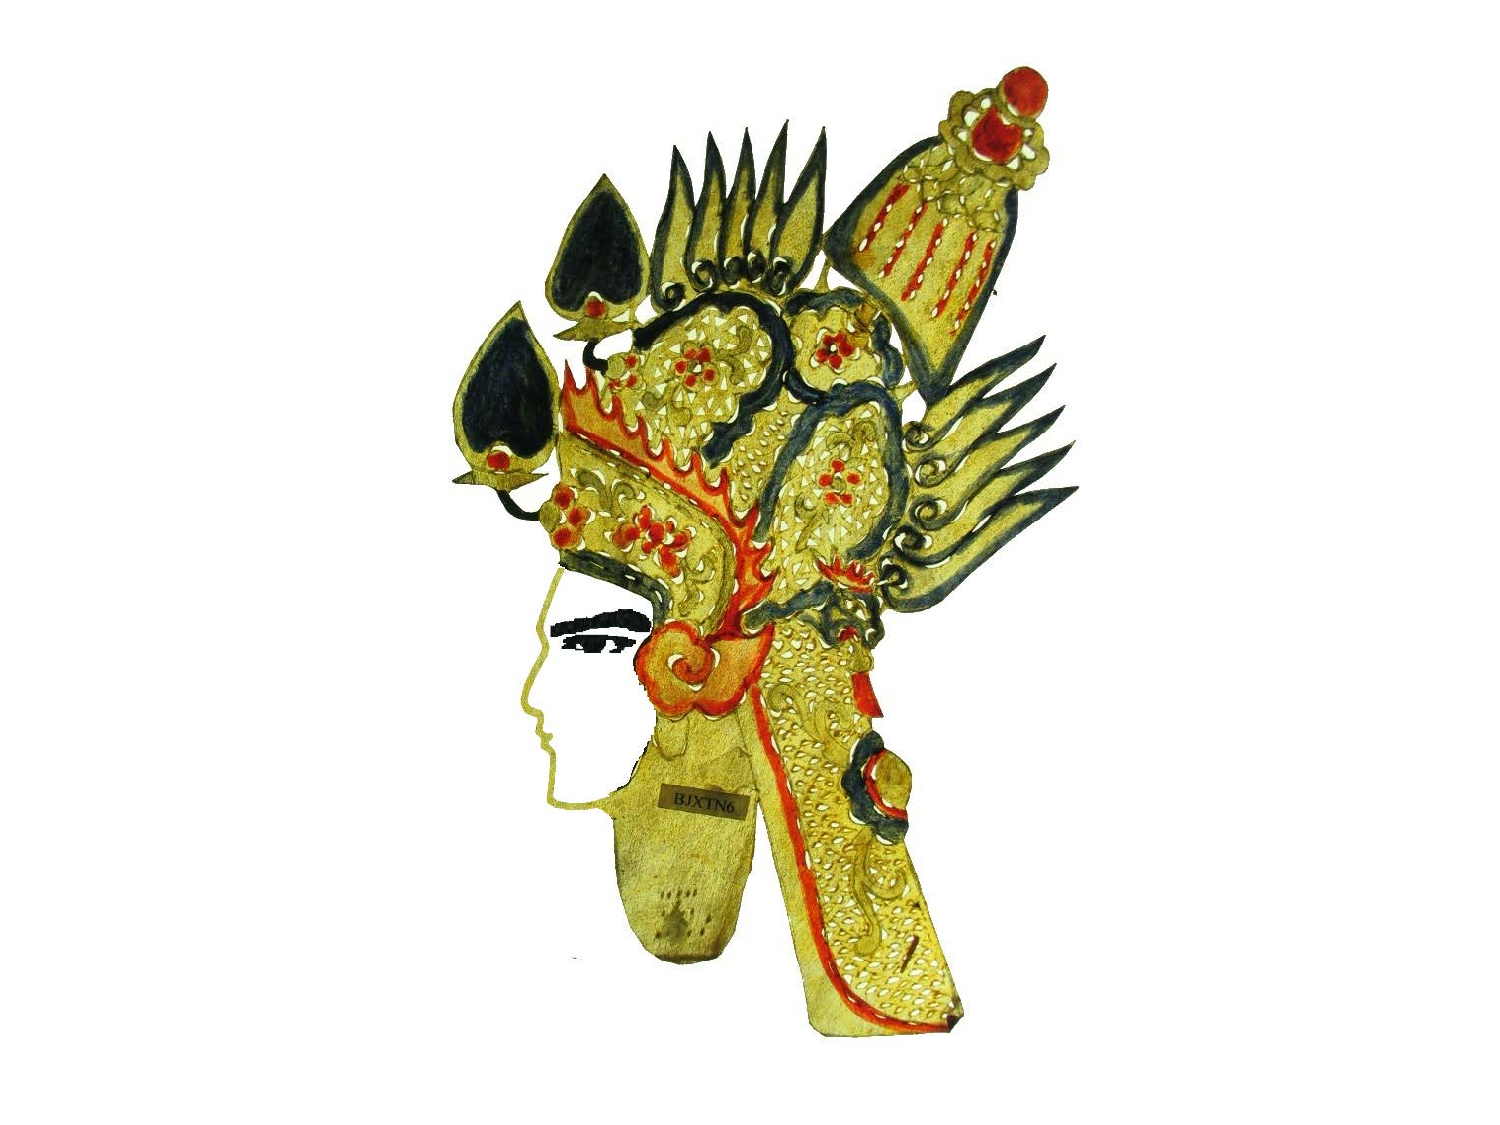
\includegraphics[scale=0.4]{figure/result_example.pdf}
\caption{\small{examples of creators}}
\label{fig:firstfig}
\end{center}
\end{figure}


\subsubsection{User Study}

Totally, 40 participants (15 females and 25 males who are students and staff members of National University of Singapore) ranged from 22 to 40 years old ($\mu$=27.3, $\sigma$=3.9) participated in the user study. Then we show some qualitative exemplar results. Finally we discuss the limitation of the system. 


\begin{itemize}
    \item Natural: Is the result image natural or with obvious artifacts? 
    \item Aesthetic: Does the result looks elegant or ugly? 
    \item Discriminative: Can you recognize the people/object inside the image?
    \item Informative: How much information does the image convey?
    \item Visual Effect: Is the result vivid? 
    \item Overall Attractiveness: All in all, do you like this system?
\end{itemize}

\begin{figure}[t]
\begin{center}
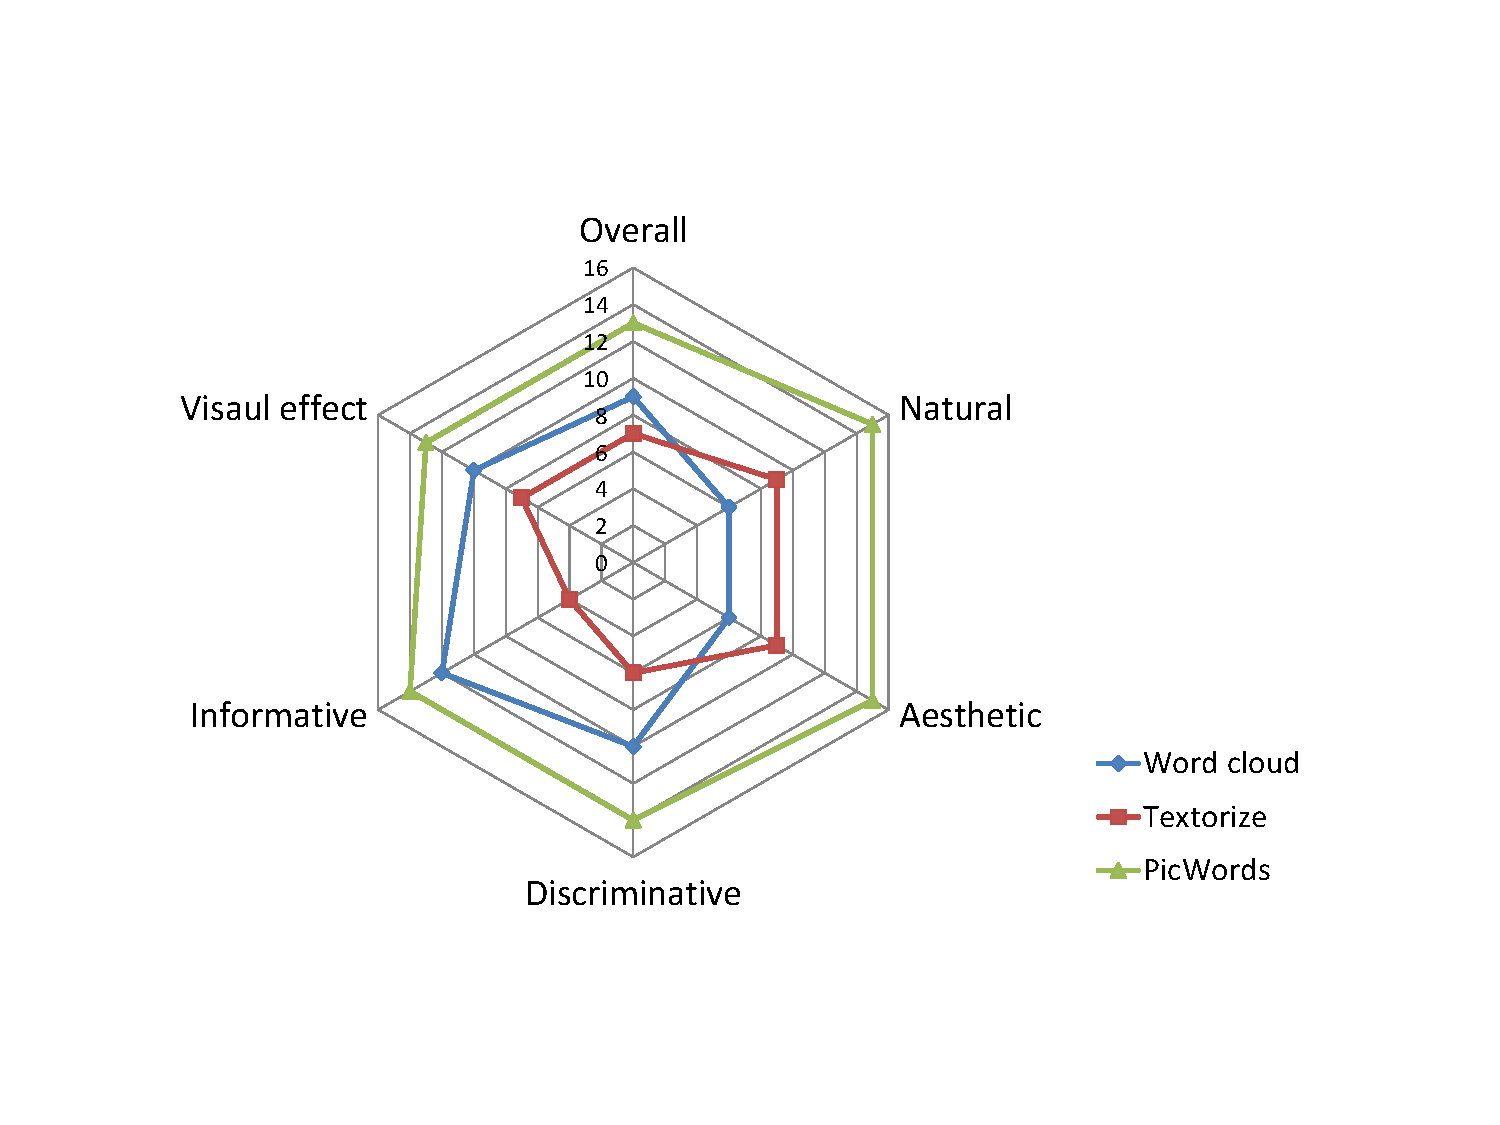
\includegraphics[scale=0.35]{figure/baseline2.pdf}
\caption{\small{user study}}
\label{fig:firstfig}
\end{center}
\end{figure}




%In this section, we first analyze the learned model, and then introduce two experiments specifically designed to evaluate the effectiveness of our model in two applications, \emph{i.e.}, clothing recommendation and clothing pairing.











\section{Conclusions} \label{sec:conclusion}






\bibliographystyle{plain}
\bibliography{puppetry}


\end{document}
